%Szablon przygotowany przez mgr Marcina Hanca, ze zmianami dr inż. Michała Rena

\documentclass[12pt,a4paper,leqno,oneside,titlepage]{book}

% amssymb musi być wczytane przed babel
\usepackage{amssymb} 
% Wczytanie pakietów: kodowania, czcionki i języki.
\usepackage[utf8]{inputenc}
\usepackage{lmodern}
\usepackage[english,polish]{babel}
% Wczytanie pakietu 'polski' w celu zapewnienia polskich nazw.
\usepackage{polski}
% Czcionki matematyczne.
\usepackage{amsfonts}
\usepackage{amsmath}
% Pakiet dodający rumuńskie znaki specjalne -- z przecinkiem pod literą.
\usepackage{combelow}
% pseudokody algorytmów
\usepackage{algorithm}
\usepackage[noend]{algpseudocode}
% Ładne początki rozdziałów (pakiet fncychap).
% Polecam Sonny i Conny. Bjornstrup najładniejszy, ale mi się bugował.
\usepackage[Sonny]{fncychap}
% Ładne i klikalne odnośniki.
\usepackage{url}
% Odnośniki dla adresów z polskimi znakami.
\usepackage[]{hyperref}
% Możliwość tworzenia łączonych pól (wg. rzędów) w tabelach.
\usepackage{multirow}
% Pakiet do cytowania kodów źródłowych.
\usepackage{listings}
% Pakiet do ładnego wstawiania grafik.
\usepackage{graphicx}
% Pakiet dodający możliwość wstawienia rozdziału "Akronimy".
\usepackage{acronym}
% Pakiet dodający kolory
\usepackage[usenames,dvipsnames,svgnames,table]{xcolor}
% Pakiet rozwiązujący problem z underscore w Section.
\usepackage[T1]{fontenc}
% Pakiet dodający definicje i twierdzenia.
\usepackage{amsthm}

\frenchspacing

\author{Magdalena Mozgawa}
\title{Ataki na systemy przetwarzania obrazu}

% \imod{k} Ładny zapis dzielenia modulo.
\makeatletter
\def\imod#1{\allowbreak\mkern10mu({\operator@font mod}\,\,#1)}
\makeatother

% \rom{n} Liczba n zapisana rzymsko.
\makeatletter
\newcommand*{\rom}[1]{\expandafter\@slowromancap\romannumeral #1@}
\makeatother

% Własne definicje.
% \begin{mydef}
%     Treść definicji.
% \end{mydef}
\newtheorem{mydef}{Definicja}

% Ładny sposób wstawiania cytatu rozpoczynającego rozdział.
% \begin{chapquote}{KTO}
%     CO ONA POWIEDZIAŁA?
% \end{chapquote}
\makeatletter
\renewcommand{\@chapapp}{}
\newenvironment{chapquote}[2][2em]
  {\setlength{\@tempdima}{#1}%
   \def\chapquote@author{#2}%
   \parshape 1 \@tempdima \dimexpr\textwidth-2\@tempdima\relax%
   \itshape}
  {\par\normalfont\hfill--\ \chapquote@author\hspace*{\@tempdima}\par\bigskip}
\makeatother

% Zmiana tekstów w listingach kodów źródłowych na j. polski.
\renewcommand\lstlistingname{Kod źródłowy}
\renewcommand\lstlistlistingname{Spis kodów źródłowych}

% Redefinicja Abstract'ów.
% W celu możliwości wstawienia dwóch na jedną stronę.
\newenvironment{abstractpage}
  {\cleardoublepage\vspace*{\fill}\thispagestyle{empty}}
  {\vfill\cleardoublepage}
\newenvironment{abstract}[1]
  {\bigskip\selectlanguage{#1}%
   \begin{center}\bfseries\abstractname\end{center}}
  {\par\bigskip}

% Dodatkowe definicje stylu stron.
\lstset{
  basicstyle={\small\ttfamily},
  breaklines=true,
  columns=flexible
}

\setlength{\oddsidemargin}{0.5in}
\setlength{\textwidth}{5.7in}
\setlength{\topmargin}{0in}
\setlength{\textheight}{8.5in}
\linespread{1.05}

% Tu rozpoczyna się zawartość pracy!
\begin{document}

% Strona tytułowa zgodna z wymaganiami:
% http://www.wmi.amu.edu.pl/pl/prace-dyplomowe
\begin{titlepage}
\let\footnotesize\small
\let\footnoterule\relax
\let \footnote \thanks

\begin{center}
{\large \bf Uniwersytet im. Adama Mickiewicza w Poznaniu \\ Wydział Matematyki i~Informatyki \par}
\vspace{0.5cm plus 1mm minus 2mm}
{{\bf Informatyka} \\%(Tu wpisz swój kierunek studiów)
\small Informatyka kto wie jaka to będzie\par}%(Tu wpisz specjalizację jeśli ją masz)
\end{center}%

\vspace{1.5cm plus 1fill}
\begin{flushleft}
{\center {\bf \Large Magdalena Mozgawa} \\ \normalsize Nr albumu: \bf 389479\par}%(Tu wpisz swoje dane)
\end{flushleft}
\vspace{1.5cm plus 1mm minus 2mm}

\begin{center}
{\huge\textbf{Ataki na systemy przetwarzania obrazu}\par}%(Tu wpisz tytuł pracy -- taki jak na porozumieniu i w systemie pd.wmi.amu.edu.pl)
\vspace{0.5cm plus 1mm minus 2mm}
{\large Attacks on computer vision systems}%(Tu wpisz angielski tytuł pracy -- taki jak na porozumieniu i w systemie pd.wmi.amu.edu.pl)
\par
\vspace{1.5cm plus 1.5fill}

\begin{flushright}\large
\begin{tabular}{l}
Praca magisterska\\[3pt]
\MakeUppercase{ }\\[3pt]
Promotor: \\[3pt]
\bfseries dr inż. Michał Ren \\[3pt]
\end{tabular}
\end{flushright}
\vspace{4cm plus .1fill}
{\large 2021 (oby)\par}%Tu wpisz rok oddania pracy
\end{center}
\end{titlepage}

% Zgłoszenie braku numerowania kolejnych stron.
\pagenumbering{gobble}

\begin{flushright}{
Poznań, dnia .....................
}\end{flushright}
\begin{center}{
\par
\vspace{1.5cm plus 1.5fill}
{\large OŚWIADCZENIE}
}\end{center}
\par
\vspace{1.5cm plus 1.5fill}%(Nie zapomniej tu wpisać danych osobowych i tytułu pracy. Wyrażanie zgody na udostępnianie pracy jest dobrowolne.)
Ja, niżej podpisany IMIONA NAZWISKO student Wydziału Matematyki i~Informatyki Uniwersytetu im. Adama Mickiewicza w Poznaniu oświadczam, że przedkładaną pracę dyplomową pt: ,,TYTUŁ PRACY'' napisałem samodzielnie. Oznacza to, że przy pisaniu pracy, poza niezbędnymi konsultacjami, nie korzystałem z pomocy innych osób, a~w~szczególności nie zlecałem opracowania rozprawy lub jej części innym osobom, ani nie odpisywałem tej rozprawy lub jej części od innych osób.\\

Oświadczam również, że egzemplarz pracy dyplomowej w~wersji drukowanej jest całkowicie zgodny z~egzemplarzem pracy dyplomowej w~wersji elektronicznej.\\

Jednocześnie przyjmuję do wiadomości, że przypisanie sobie, w~pracy dyplomowej, autorstwa istotnego fragmentu lub innych elementów cudzego utworu lub ustalenia naukowego stanowi podstawę  stwierdzenia  nieważności postępowania w~sprawie nadania tytułu zawodowego.\\

Wyrażam zgodę na udostępnianie mojej pracy w czytelni Archiwum UAM.\\

Wyrażam zgodę na udostępnianie mojej pracy w zakresie koniecznym do ochrony mojego prawa do autorstwa lub praw osób trzecich.
\par
\vspace{1.5cm plus 1.5fill}
\begin{center}{
..............................................\\
{\footnotesize(czytelny podpis studenta)}
}\end{center}

\newpage

\phantom{.}

%Zastanów się komu chcesz podziękować; oczywiście dla siebie możesz stworzyć wiele wersji pracy z różnymi podziękowaniami dla rodziny, znajomych, szefa... Te podziękowania są przykładem i naprawdę możesz coś z siebie wykrzesać.
\vspace{12cm} \hspace{1cm}\phantom{.}\\
\phantom{.}\hspace{5cm}{Tutaj będą podziękowania dla sąsiadów}\\
\phantom{.}\hspace{5cm}{za siedzenie cicho.}\\
\phantom{.}\hspace{5cm}{}\\
\phantom{.}\hspace{5cm}{I coś dla promotora.}\\

\newpage
% Przód pracy - spisy i abstrakty.
\frontmatter
% Spis treści ze specjalnym uwzględnieniem podkreśleń w tytułach sekcji.
\pagestyle{plain}
{
    \catcode`\_=12
    \tableofcontents
} 
% Spis ilustracji -- możesz mieć, ale nie musisz.
\listoffigures
% Spis tabeli -- możesz mieć, ale nie musisz.
\listoftables
% Spis listingów kodów źródłowych -- możesz mieć, ale nie musisz.
\begingroup
\let\clearpage\relax
\lstlistoflistings
\endgroup

% Strona z abstraktami.
\begin{abstractpage}
% Abstrakt w języku polskim.
\begin{abstract}{polish}
Streszczenie wstępu jest dobrym pomysłem na początek abstraktu. Dobre praktyki tworzenia abstraktów znajdują się np. na stronie\footnote{
\url{http://www.editage.com/insights/how-to-write-an-effective-title-and-abstract-and-choose-appropriate-keywords}}.
Wczuj się w rolę informatyka, który będzie czytał sam abstrakt, żeby zdecydować, czy reszta pracy mu się przyda. Zwięzłość jest w cenie, niemniej jednak trzeba się starać opisać o czym głównie jest praca, jak również co jest w tej pracy szczególnego, czego nie można znaleźć w innych. Zwykle abstrakt pisze się po napisaniu pracy, myśląc o takich kwestiach jak np. ,,jaki problem próbowano rozwiązać'', ,,jaka była motywacja skupienia się nad tym problemem'', ,,za pomocą jakich środków cel został osiągnięty''. Wiele abstraktów różnego rodzaju prac można obejrzeć w Internecie.
\end{abstract}
\smallskip
\noindent \textbf{Słowa~kluczowe:} praca dyplomowa, wzór, przewodnik

%Abstrakt w języku angielskim.
\begin{abstract}{english}
Translation of your Polish abstract. Some leeway is allowed, but make sure it is a translation, not a completely different abstract. If you have a problem with English, ask your supervisor to help you translate. Machine translations (e.g. Google translate) are not good enough (yet...) to be acceptable.
\end{abstract}
\smallskip
\noindent \textbf{Keywords:} thesis, template, guide
\end{abstractpage}

% Finally - PRACA!
\mainmatter

% Wstęp jest uwzględniony w spisie treści jako rozdział bez numeru.
\addcontentsline{toc}{chapter}{Wstęp}
\chapter*{Wstęp}

Krótkie omówienie tego, o czym będzie praca. (Czyli co zostanie w pracy powiedziane.)

Rzeczy które tu można ująć to np. 
\begin{itemize}
\item mini-przewodnik po własnych wynikach, czy że zrobiono to, tamto i owamto
\item motywacja do pracy, czyli dlaczego się tym zajęto i dlaczego masa rzeczy już na ten temat napisanych nie wystarczyła do szczęścia
\item omówienie struktury pracy, czyli w tym rozdziale jest to, a tym owo
\item historia badań na podobnymi tematami i aktualny stan wiedzy
\end{itemize}

Ilu autorów, tyle wstępów\ldots{} Nie traktuj powyższych elementów jako obowiązkowe.

\chapter{Systemy przetwarzania obrazu}%Na końcu tytułów rozdziałów i podrozdziałów nie stawiamy kropek.

Czego NIE opisuję w tym rozdziale (póki co): dlaczego redukować w ogóle wymiarowość obrazów ("przekleństwo wymiarowości")), jak wygląda pipeline przetwarzania danych (ekstrakcja cech-deskryptorów, trenowanie modelu, testowanie modelu)).

%
%
%
%
%
%
%
%
% HOG
%
%
%
%
%
%
%
%
%
%
\section{Histogramy zorientowanych gradientów}

Histogramy zorientowanych gradientów (ang. \textit{histograms of oriented gradients}, dalej: HOG) to deskryptory pozwalające na opisanie zawartości danego obrazu za pomocą wielkości i orientacji gradientów. Technika ta pozwala na redukcję wymiarowości obrazu oraz zniwelowanie wpływu lokalnych różnic na całość deskryptora\cite{DalalTriggs05Hog}.

\subsection{Opis algorytmu}
Algorytm tworzenia histogramów zorientowanych gradientów składa się z dwóch faz: wyliczenia gradientów oraz głosowania histogramów. Pierwsza pozwala na pozyskanie dla $n\times m$-wymiarowego obrazu w skali RGB dwóch $n\times m$-wymiarowych macierzy opisujących gradienty w tym obrazie. Druga korzysta z tych macierzy do wyznaczenia histogramów zorientowanych gradientów w celu dalszej redukcji wymiarowości obrazu. Fazy te zostały bardziej szczegółowo opisane poniżej.

\paragraph{Wyliczenie gradientów.}
Plikiem wejściowym jest analizowany obraz o wymiarach $n\times m$ pikseli, który jest przetwarzany do 8-bitowej skali szarości i dzielony na nakładające się komórki (ang. \textit{cells}) ustalonej wielkości, wyznaczone wokół centralnego piksela danej komórki. Następnie dla każdej takiej komórki wylicza się wielkość ($M(x,y)$) i kąt ($\alpha(x,y)$) wektora gradientu:

\begin{align}
M(x,y) = \sqrt{\left( x^{2}+x^{2}\right)} \\
\alpha(x,y) = \arctan{\frac{x}{y}}
\end{align}

gdzie dla centralnego piksela danej komórki, znajdującego się w $i$-tej kolumnie $j$-tego wiersza, $x$ i $y$ to wartość bezwględna różnicy wartości między najodleglejszymi pikselami odpowiednio w $j$-tym wierszu i $i$-tej kolumnie. Uzyskuje się w ten sposób dwie macierze $n\times m$ z wartościami odpowiadającymi wielkościom gradientów oraz ich kątom \textit{modulo} $180^\circ$\cite{dpi2008}.

\paragraph{Głosowanie histogramu.}
Elementem wejściowym są macierze uzyskane w kroku pierwszym. Macierze są dzielone na nienakładające się bloki (ang. \textit{blocks}). Następie w obrębie każdego bloku odbywa się głosowanie, którego wynikiem jest histogram danego bloku. Szczegółowy algorytm głosowania pokazano w pseudokodzie.

\begin{algorithm}
\caption{Głosowanie histogramu w bloku}
\hspace*{\algorithmicindent} \textbf{Wejście:} $B_{k}$ -- blok kątów w postaci listy \textit{i}-elementowej, $B_w$ -- blok wielkości gradientów w postaci listy \textit{i}-elementowej. \\
\hspace*{\algorithmicindent} \textbf{Wyjście: } \textit{H} -- 9-elementowa lista definiująca histogram o klasach $0-20^{\circ}$, $20-40^{\circ}$, ..., $160-0^{\circ}.$ 

\begin{algorithmic}
\State $H\gets [0, 0, 0, 0, 0, 0, 0, 0, 0]$
\For{$i\gets 1, n$}
  \State $c\gets \left\lfloor{B_{k_{i}}}\right\rfloor$
  \State $h\gets c\div 20$
  \If {$c==B_{k_{i}}$}
    \State $H[h]\gets B_{w_{i}}\div 2$
    \State $H[h-1]\gets B_{w_{i}}\div 2$
  \Else
    \State $H[h]\gets B_{w_{i}}$
  \EndIf
\EndFor
\end{algorithmic}
\end{algorithm}

\paragraph{Efekt końcowy.}
Wynikiem działania zastosowanej metody są histogramy zorientowanych gradientów. Warto zauważyć, że użycie tej metody prowadzi do znacznego zmniejszenia wymiarowości danych. Przykładowo, można policzyć, że 24-bitowy obraz o wymiarach $64\times128$ pikseli, do którego opisania pierwotnie potrzeba by 24 576 wartości, może być podzielony na 27 bloków $16\times16$ pikseli, co daje 243 wartości w histogramach opisujące cały obraz. Jest to ponad stukrotne zmniejszenie liczby wartości opisujących obraz, które wciąż pozwala na stworzenie stosunkowo skutecznego deskryptora\cite{DalalTriggs05Hog}.

\subsection{Klasyfikatory oparte o histogramy zorientowanych gradientów}

Wyliczenie deskryptora dla wielu obrazów to pierwszy krok do stworzenia klasyfikatora danej cechy opartego o uczenie maszynowe. Popularność HOG przypada na wczesne lata 2000, kiedy znacznym poważaniem cieszyły się m.in. maszyny wektorów podpierająch (ang. \textit{Support Vector Machines}, dalej: SVM). Jest to model uczenia maszynowego, zaproponowany przez Vladimira Vapnika w 1995, pozwalający na wyznaczenie optymalnej hiperpłaszczyzny, która odziedzialałaby dane z różnych klas zachowując największy możliwy margines zaufania \cite{Norbert03,Vapnik95}. Ten model został zastosowany również przez autorów metody histogramów zorientowanych gradientów, jednak jego bardziej szczegółowe omówienie wykracza poza zakres tej pracy i nie jest konieczne do zrozumienia sposobu działania metody ani możliwych dróg ataku na nią \cite{DalalTriggs05Hog}. (KOMENTARZ Chyba że promotor bardzo będzie tego chciał albo zabraknie materiału.)

Wytrenowany klasyfikator może zostać następnie zastosowany do wykrywania danej cechy na różnych zdjęciach, także takich, które nie były użyte do jego wytworzenia. Przykładem klasyfikatora, którego można użyć do wykrycia twarzy \textit{en face} jest ten załączony do biblioteki \textit{dlib}, otwartoźródłowej biblioteki z narzędziami do uczenia maszynowego, napisanej w języku C++ i posiadającej też API do języka Python\cite{dlibPage}. Poniżej zaprezentowano przykładową implementację wspomnianego klasyfikatora w celu rozpoznania twarzy na zdjęciu oraz efekt działania takiego skryptu.

\lstinputlisting[language=Python, label={lst:hog} captionpos=b, belowcaptionskip=4pt, caption={Wyszukiwanie twarzy z użyciem biblioteki dlib}]{hog_classifier.py}

\begin{figure}[!tbp]
  \centering
  \begin{minipage}[b]{0.4\textwidth}
    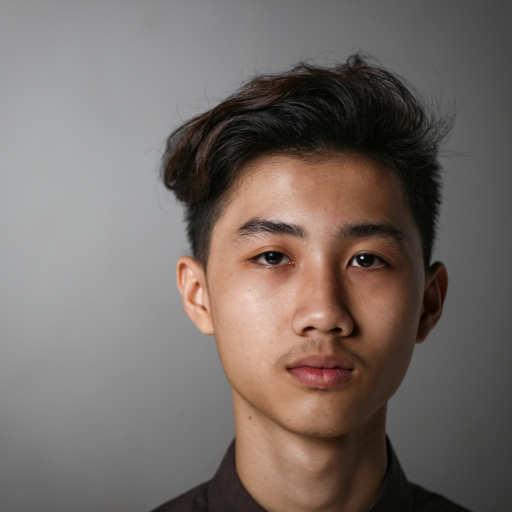
\includegraphics[width=\textwidth]{pictures/face.jpg}
    \caption{Oryginalne zdjęcie.\cite{Putera}}
  \end{minipage}
  \hfill
  \begin{minipage}[b]{0.4\textwidth}
    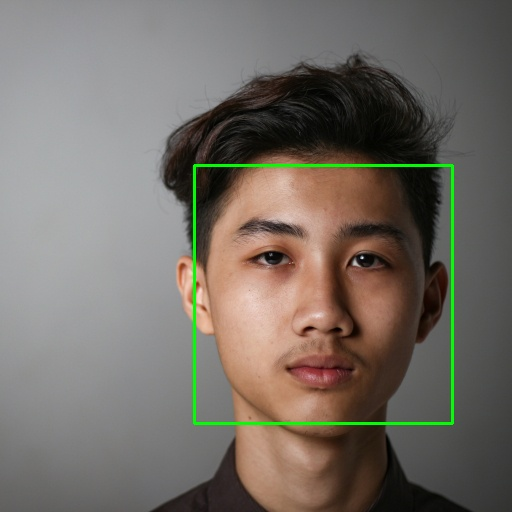
\includegraphics[width=\textwidth]{pictures/face_detected.jpg}
    \caption{Efekt działania klasyfikatora.}
  \end{minipage}
\end{figure}

%
%
%
%
%
%
% Viola-Jones
%
%
%
%
%

\section{Metoda Viola-Jonesa}

Metoda Viola-Jonesa to czteroetapowy framework pozwalający na wykrywanie określonych cech na zdjęciach, na przykład odnajdowanie na nich twarzy ludzi, określonych zwierząt czy obiektów. Celem tej sekcji jest opisanie jego poszczególnych etapów: wyboru cech Haara, stworzenia obrazu integralnego (ang. \textit{Integral Image}), wyboru cech do klasyfikatora w oparciu o zmodyfikowaną wersję algorytmu AdaBoost i wreszcie konstrukcji kaskady klasyfikatorów.\cite{ViolaJones01}

\subsection{Wybór cech Haara}
Podstawę klasyfikacji w metodzie Viola-Jonesa stanowią prostokątne cechy, czyli grupy pikseli o określonym ułożeniu. Cechy te, ze względu na podobieństwo do falek Haara, nazywane są cechami Haara (ang. \textit{Haar-like features}). Metoda zaproponowana przez autorów zakłada skorzystanie z trzech rodzajów cech (patrz Rysunek \ref{fig:haar_features}):
\begin{itemize}
	\item dwuprostokątnej cechy (ang. \textit{two-rectangle feature}), czyli różnicy między sumami pikseli w dwóch prostokątach o tym samym rozmiarze i kształcie, przylegających do siebie w pionie lub w poziomie,
	\item trójprostkątnej cechy (ang. \textit{three-rectangle feature}), czyli różnicy sumy dwóch zewnętrznych prostokątów i środkowego prostokąta,
	\item czteroprostokątnej cechy (ang. \textit{four-rectangle feature}), czyli różnicy między parami prostokątów znajdującymi się na poprzecznej.
\end{itemize}

W praktyce cechy Haara przekazują informacje dotyczące kontrastów między prostokątnymi grupami pikseli. Pozwala to wyznaczyć obszary, które są względem siebie jaśniejsze lub ciemniejsze. W przypadku wykrywania twarzy, cechy mogą odpowiadać różnicom w układaniu się światła i cienia na twarzy, na przykład między mostkiem nosa a oczami albo między oczami a policzkami.

Detektor zastosowany przez autorów ma 24x24 piksele, co w przeliczeniu daje zbiór ponad 180000 cech różnych rodzajów i wymiarów. Same operacje arytmetyczne potrzebne do wyliczenia tych cech stanowić mogą spore wyzwanie (jeszcze większe stanowiły na początku lat 2000, gdy algorytm powstawał), dlatego autorzy opracowali metodę przedstawioną w kolejnej sekcji: wyliczanie formy pośredniej w postaci obrazu integralnego.\cite{ViolaJones01}

\begin{figure}[!tbp]
  \centering
  \begin{minipage}[b]{0.9\textwidth}
    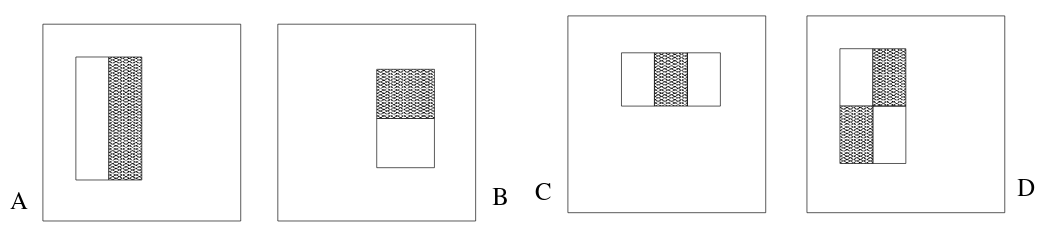
\includegraphics[width=\textwidth]{pictures/Haar_features.png}
    \caption{Cechy Haara: (A) i (B) to cechy dwuprostokątne, (C) ~--- cecha trójprostokątna, (D) ~--- czteroprostokątna.\cite{ViolaJones01}}
    \label{fig:haar_features}
  \end{minipage}
\end{figure}

\subsection{Tworzenie obrazu integralnego}

W celu usprawnienia wyliczeń wartości cech Haara używa się pośredniej formy obrazu, czyli tzw. obrazu integralnego (ang. \textit{integral image}). Jego wartość w pozycji o współrzędnych \textit{x, y} zawiera sumę pikseli ponad i na lewo od \textit{x, y}, włącznie z samymi \textit{x, y}:
\begin{align}
ii(x,y) = \sum_{x'\leqslant x, y' \leqslant y} i(x', y'),
\end{align}
gdzie $ii(x,y)$ to obraz integralny, a $i(x,y)$ to oryginalny obraz. Korzystając z rekurencji możliwe jest wyliczenie obrazu integralnego w ramach pojedyńczego przejścia przez oryginalny obraz. Następnie, używając obrazu integralnego, obliczać można sumy pikseli w określonych prostokątach korzystając z poprzedzających je obszarów. Metoda ta została pokazana w ilustracji \ref{fig:integral_image_sums}.

\begin{figure}[!tbp]
  \centering
  \begin{minipage}[b]{0.4\textheight}
    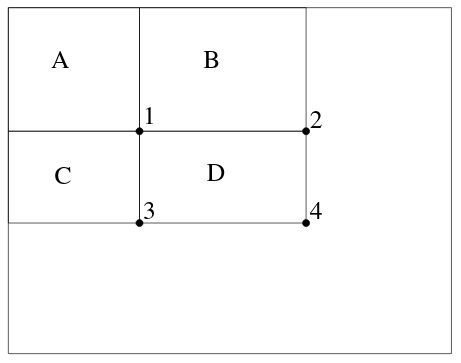
\includegraphics[width=\textwidth]{pictures/integral_image_sums.png}
  \end{minipage}
  \caption{Sumę pikseli w prostokącie D można wyliczyć w odniesieniu do do pól A, B i C. Wartość w punkcie 1 jest równa sumie pikseli w prostokącie A, w punkcie 2 ~--- A + B, w punkcie 3 ~--- A + C, w punkcie 4 ~--- A + B + C + D. Wobec tego suma D wynosi D + A - (B + C).\cite{ViolaJones01}}
  \label{fig:integral_image_sums}
\end{figure}

Skorzystanie z obrazu integralnego pozwala na dużo sprawniejsze wyznaczenie cech, na postawie których zostanie zbudowany klasyfikator.

\subsection{Wybór cech}

Jak wcześniej wspomniano, dla zastosowanego detektora 24x24 piksele uzyskuje się zbiór ponad 180000 cech o różnej użyteczności. Żeby wyznaczyć tę użyteczność i wybrać z tego zbioru cechy przydatne do wykrycia określonego typu obiektu korzysta się ze zmodyfikowanej wersji algorytmu AdaBoost. Tylko użyteczne cechy trafiają później do klasyfikatora. Cechy te w pojedynkę mogą być stosunkowo słabymi predyktorami wyniku klasyfikacji, dlatego taki rodzaj uczenia nosi też nazwę algorytmu słabych klasyfikatorów. Eksperymenty autorów wykazały, że stosunkowo niewielka liczba takich cech jest w stanie stworzyć efektywny klasyfikator i dlatego głównym wyzwaniem jest odnalezienie owych cech.
Stworzona przez autorów modyfikacja AdaBoost ma za zadanie wybrać cechy dające najniższy wskaźnik błędów. Dla każdej z cech, klasyfikator  ustala optymalny próg funkcji klasyfikującej, taki że minimalna liczba przykładów treningowych zostaje zaklasyfikowana niepoprawnie:

\begin{align}
h_{j}(x) = \left.
	\begin{cases}
		x  & \text{jeśli } p_{j}f_{j}(x) \leq p_{j}\theta_{j} \\
		-x & \text{w innym przypadku}
	\end{cases}
	\right.
\end{align}

gdzie $x$ to 24x24-pikselowe podokno obrazu, $h_{j}(x)$ - klasyfikator, $f_{j}$ - cecha, $\theta_{j}$ - próg i $p_{j}$ - znak liczby. Dokładniejszy opis zmodyfikowanego algorytmu AdaBoost znajduje się w algorytmie x. W praktyce żadna cecha nie jest w stanie w pojedynkę dokonać klasyfikacji z odpowiednio dużą dokładnością. W opisywanym przypadku współczynniki błędu cech wybranych w pierwszych rundach wynosiły między 0,1 a 0,3, później dochodząc do 0,4 i 0,5 (czyli aż do wyniku losowego rzutu monetą).\cite{ViolaJones01}

\subsection{Konstrukcja kaskady klasyfikatorów}

Celem konstrukcji kaskady klasyfikatorów jest stworzenie systemu, który łączy wyższą skuteczność i krótszy czas przetwarzania obrazów. Autorzy posłużyli się mechanizmem, w którym klasyfikatory ustawia się w odpowiedniej kolejności. Najpierw umieszcza się prostsze klasyfikatory, które odrzucają jak najwięcej negatywnych przypadków (akceptując przy tym potencjalną dużą liczbę błędów pierwszego rodzaju), a następnie stosuje się bardziej złożone klasyfikatory, które służą odsianiu błędów pierwszego rodzaju. Finalnie uzyskuje się drzewo decyzyjne — kaskadę, ang. \textit{cascade} — o specyficznym, "zdegenerowanym" kształcie: każdy węzeł nie będący węzłem końcowym ma dwie gałęzie, przy czym tylko jedna z tych gałęzi ma swoje dwie gałęzie, itd.

Kolejność umieszczenia klasyfikatorów oraz ich liczba są wyznaczane w procesie trenowania kaskady. Ze względu na trudność ułożenia odpowiednich klasyfikatorów w odpowiedniej kolejności przy jednoczesnym spełnieniu założeń dotyczących skuteczności i wydajności (im więcej cech ma klasyfikator, tym jest dokładniejszy i mniej wydajny) stosuje się prostą heurystykę, żeby otrzymać "dość dobrą" kaskadę. Początkowo określa się finalną pożądaną dokładność klasyfikatora oraz akceptowalny odsetek błędów pierwszego rodzaju. Na każdym etapie kaskady dany klasyfikator ma za zadanie redukcję liczby błędów pierwszego rzędu (co jednocześnie może zmniejszać dokładność). Na początku etapu wybiera się dwie wartości docelowe: minimum o jakie chce się zmniejszyć liczbę błędów pierwszego rodzaju oraz maksimum o jakie chce się zmniejszyć dokładność klasyfikatora. Na podstawie tych wytycznych trenuje się kaskadę, dobierając cechy do momentu uzyskania wybranych wartości. Klasyfikator, który odniósł sukces w tym etapie jest dopisywany do całej kaskady, a trening przechodzi do kolejnego etapu z nowymi wartościami docelowymi. Etapy są dodawane, dopóki nie stworzy się kaskady o parametrach odpowiadających początkowym wymaganiom.

W eksperymentach autorów kompletna kaskada klasyfikatorów, używana do wykrywania twarzy \textit{en face} (and. \textit{frontal face classifier}), składała się z 38 etapów i 6061 cech. Na ówczesnym sprzęcie (procesor Pentium III 700 MHz) pozwalała ona na kilkanaście razy szybsze przetwarzanie obrazów niż istniejące rozwiązania, nie odbiegając od nich negatywnie odsetkiem błędów pierwszego rodzaju.\cite{ViolaJones01}

%
%
%
%
%
%
% CNNs
%
%
%
%
%

\section{Konwolucyjne sieci neuronowe}

Konwolucyjne sieci neuronowe (ang. \textit{convolutional neural networks}, także: \textit{CNN(s)}) to specjalistyczny rodzaj sieci neuronowych, których zadaniem jest przetwarzanie danych o określonej strukturze (zwykle jest to 1- lub 2-wymiarowa siatka), np. szeregów czasowych czy obrazów. Ich nazwa bierze się z tego, że co najmniej jedna z warstw w CNN musi zawierać warstwę konwolucyjną, czyli dokonywać przekształcenia danych poprzez zastosowanie konwolucji.\cite{Goodfellow-et-al-2016} Celem tej sekcji jest opisanie teorii stojącej za konwolucyjnymi sieciami neuronowymi i pojęć im towarzyszących, takich jak metoda gradientu prostego, propagacja wsteczna i różne rodzaje warstw występujących w CNNach.

\subsection{Metoda gradientu prostego}

Wiele algorytmów używanych w głębokim uczeniu maszynowym korzysta z metod optymalizacji numerycznej, czyli odnajdowania minimum lub maksimum danej funkcji $f(x)$ poprzez manipulowanie argumentem funkcji. Jedną z takich metod jest metoda gradientu prostego, korzystająca z wartości pochodnej z $f(x)$ w danym punkcie do określenia "w którą stronę" należy przesunąć $x$ w celu zbliżenia się do lokalnego minimum funkcji $f(x)$. W praktyce ze względu na ogromną przestrzeń, jaką należałoby przeszukać w celu znalezienia optymalnego $x$, liczba testów kolejnych jego wartości musi być ograniczona. Analogią dla tego procesu jest schodzenie w dół zbocza z perspektywą zapadającego zmroku: podróżujący musi wtedy podążać w kierunku obniżania się zbocza, ale nie może się też zatrzymywać za często w celu pomiaru, bo zastanie go zmrok.

\begin{figure}[!tbp]
  \centering
  \begin{minipage}[b]{0.5\textheight}
    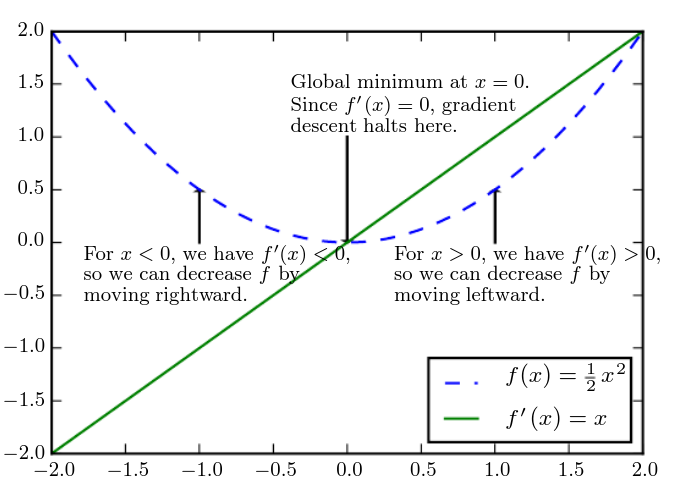
\includegraphics[width=\textwidth]{pictures/gradient_descent.png}
  \end{minipage}
  \caption{Ilustracja działania metody gradientu prostego. Pochodna funkcji $f$ w punkcie $x$ jest używana do określania kształtu funkcji.\cite{Goodfellow-et-al-2016}}
  \label{fig:gradient_descent}
\end{figure}

Dodatkowym problemem w poszukiwaniu minimów (maksimów) funkcji jest to, że może mieć ona wiele lokalnych minimów, jak również punkty siodłowe, nieodpowiadających globalnym minimom (maksimom). Jest to częsty problem w funkcjach używanych w uczeniu maszynowym. Dlatego też dobrą praktyką jest poszukiwanie "dość dobrych" wartości $f$ — wystarczająco niskich (wysokich) dla osiągnięcia pożądanej dokładności, ale niekoniecznie stanowiących minima (maksima) w znaczeniu formalnym. Przykład pokazano na Rysunku \ref{fig:approximate_minimization}. W praktyce funkcje używane w głębokim uczeniu maszynowym przyjmują wiele zmiennych, tak więc "dość dobre" wartości są wyszukiwane z użyciem pochodnych cząstkowych. Gradient funkcji $f$ jest wówczas rozumiany jako wektor zawierający wszystkie pochodne cząstkowe i oznaczany przez $\nabla_{x}f(x)$.\cite{Goodfellow-et-al-2016}


\begin{figure}!tbp]
  \centering
  \begin{minipage}[b]{0.5\textheight}
    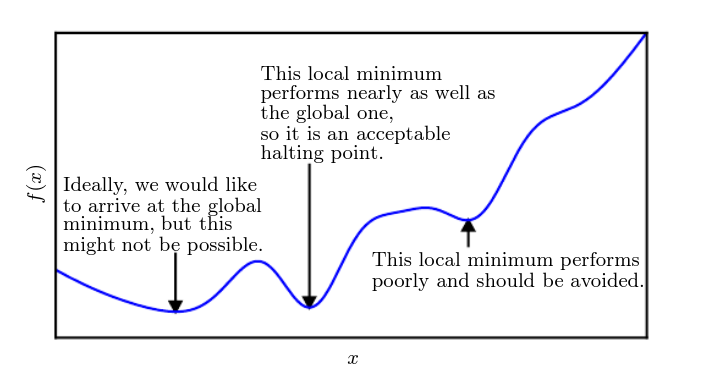
\includegraphics[width=\textwidth]{pictures/approximate_minimization.png}
  \end{minipage}
  \caption{Odnajdywanie "wystarczająco dobrej" wartości $x$. Choć wartość znaleziona (np. środkowa) może nie być globalnym minimum (po lewej), to będąc dostatecznie bliską globalnemu minimum jest wystarczająca. Niedostatecznie dobra jest wartość po prawej (lokalne minimum), zbyt odbiegająca od globalnego minimum.\cite{Goodfellow-et-al-2016}}
  \label{fig:approximate_minimization}
\end{figure}

\subsection{Propagacja wsteczna}

%
%
%
%
%
% ROZDZIAŁ DRUGI
%
%
%
%
%

\chapter{Taksonomia ataków na uczenie maszynowe}

Ten rozdział zajmuje się opisem taksonomii ataków, w oparciu o NISTa (https://nvlpubs.nist.gov/nistpubs/ir/2019/NIST.IR.8269-draft.pdf) oraz "Hakowanie uczenia maszynowego".

%
%
%
%
%
% ROZDZIAŁ TRZECI
%
%
%
%
%

\chapter{Praktyczne metody ataków na systemy przetwarzania obrazu}


\subsection{Metody ataku}
Ze względu na ich stosunkowo niski poziom skomplikowania i wysoką intepretowalność w porównaniu do modeli opartych o głębokie uczenie maszynowe istnieją metody pozwalające na wizualizację deskryptorów HOG. Metody te, poza ułatwianiem pracy nad debugowaniem istniejących modeli, mogą także służyć do opracowywania metod ataku. Przegląd istniejącej literatury wskazuje, że rozwiązania oparte o HOG są podatne na dwa typy ataków: ataki przez unikanie (ang. \textit{evasion attacks}) oraz ataki przez zatrucie (ang. \textit{poisoning attacks})\cite{Hoggles, MacDonald19}. (KOMENTARZ: szersza charakterystyka typów ataków oparta o proponowaną przez NIST nomenkulaturę znajdzie się gdzieś we wstępnym rozdziale.)

\paragraph{Ataki przez unikanie.}
W przypadku HOG ataki przez unikanie polegają na przesłonięciu w obiekcie fragmentu lub fragmentów odpowiadających blokom o znaczących wartościach deskryptora. Przykładowo, w przypadku opartego o HOG detektora twarzy we wspomnianej bibliotece dlib, skuteczność wykrywania znacząco spada dla twarzy w ciemnych okularach: dla zbioru, na którym trenowany był dlibowski \textit{frontal face detector} wynosi 91\% dla ogółu zdjęć oraz 57\% dla zdjęć osób w ciemnych okularach zasłaniających oczy (niezależnie od kształtu okularów).\footnote{.(KOMENTARZ: osoba pisząca wyjęła sobie te dane z d...obrze napisanego skryptu, który przeiterował przez wszystkie obrazy oraz przez podgrupę obrazów z osobami w dość ciemnych okularach. Czy to materiał do jakiegoś appendixu?) } Podobny efekt można uzyskać dzięki założeniu np. maseczki albo komina zasłaniającego dolną część twarzy\cite{dlibPage, MacDonald19}.

\begin{figure}[!tbp]
  \centering
  \begin{minipage}[b]{0.4\textwidth}
    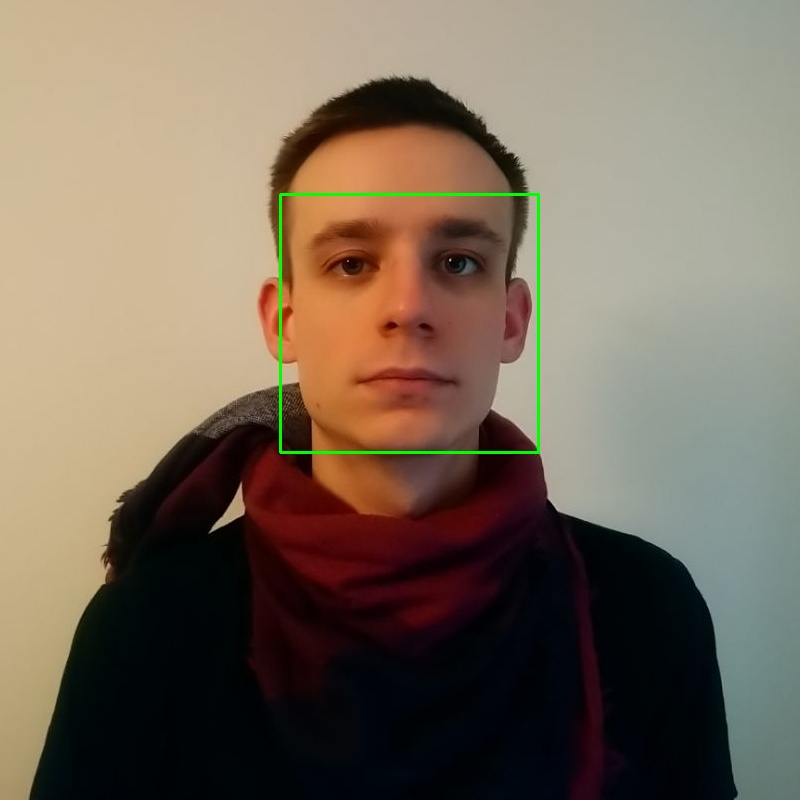
\includegraphics[width=\textwidth]{pictures/Tomek_detected.jpg}
  \end{minipage}
  \hfill
  \begin{minipage}[b]{0.4\textwidth}
    
\includegraphics[width=\textwidth]{pictures/Tomek_szalik_detected.jpg}
  \end{minipage}
  \caption{Atak przez unikanie. Źródło zdjęcia: opracowanie własne.}
\end{figure}

\paragraph{Ataki przez zatrucie.}
Innym sposobem na przechytrzenie systemu przetwarzania obrazu jest zwizualizowanie wyuczonego detektora (jeśli mamy do niego dostęp) albo histogramu gradientów dla pozytywnego przykładu, a następnie użycie go do ,,zatrucia'' materiału testowego poprzez np. zapozowanie w ubraniu z nadrukiem pokazującym tę wizualizację. W takim przypadku system popełniałby błędy pierwszego rodzaju, odnajdując poszukiwane obiekty na zdjęciach, które mogłyby ich wcale nie zawierać. Ataki przez zatrucie mogą też być połączone z atakami przez unikanie: przykładowo, w przypadku systemów wymagających, by na zdjęciu znalazła się jakaś twarz i docinających do niej zdjęcie, założenie maseczki z ,,zatrutym'' wzorem skutkowałoby jednoczesnym uniknięciem wykrycia właściwej twarzy na zdjęciu i zapamiętaniem materiału błędnego z punktu widzenia człowieka\cite{MacDonald19}. (KOMENTARZ: tutaj też będzie twarzowe zdjęcie, ale ze względu na braki drukarkowe pojawi się później.)

%
%
%
%
%
% ROZDZIAŁ CZWARTY ?
%
%
%
%
%

\chapter{Atak na popularne systemy wykrywania twarzy}

\newpage
% Dodanie wpisu Bibliografia do Spisu Treści.
\addcontentsline{toc}{chapter}{Bibliografia}
% Styl bibliografii: unsrt lub plain
\bibliographystyle{plain}
\bibliography{bibliografia}

% W przypadku dodawania dodatków:
\appendix
\addcontentsline{toc}{chapter}{Dodatki}

% Pojedynczy dodatek
\addcontentsline{toc}{section}{Dodatek A: Cośtam dodatkowego}
\chapter*{Dodatek A: Cośtam dodatkowego}

Dodatki zawierają treści, których zrozumienie nie jest konieczne do zrozumienia pracy i które mogłyby niepotrzebnie zajmować miejsce. Czasem są to listingi programów -- może np. w pracy wystarczą krótkie fragmenty do których się akurat odnosimy, a w dodatku może być cały kod źródłowy, itp.

% Spis akronimów użytych w pracy -- można mieć, ale nie trzeba; większość prac nie ma.
\chapter*{Akronimy}
\begin{acronym}
\acro{KISS}{Keep It Simple Stupid}
\acro{IT}{Information Technology}
\end{acronym}
\end{document}
